\chapter{Apprendimento automatico}\label{chap:AI_ML}
In questo capitolo si introducono i principali problemi e le principali tecniche risolutive nel campo dell'apprendimento automatico.
Nel~\Cref{sec:imparare_dai_dati} si definisce il termine apprendimento automatico; nel~\Cref{sec:tipi_problemi_ml} si categorizzano i principali problemi di apprendimento automatico; nel~\Cref{sec:valutazione_modelli} si descrivono le principali metriche di valutazione dei modelli di apprendimento automatico; nel~\Cref{sec:model_selection} si descrivono le principali tecniche per selezionare i migliori iperparametri per addestrare un modello su un certo \emph{dataset}; nel~\Cref{sec:comuni_approcci_risolutivi} si descrivono i più comuni approcci risolutivi; nel~\Cref{sec:bias_variance_tradeoff} si introduce infine la problematica dell'\emph{overfitting}/\emph{underfitting}; 

\section{Imparare dai dati}\label{sec:imparare_dai_dati}
Risolvere un problema utilizzando un computer richiede un algoritmo, una sequenza di passi da poter implementare ed eseguire. 
Per alcuni problemi sono noti uno o più algoritmi in grado di trovare soluzioni: ordinare una sequenza di numeri, per esempio, è un compito per cui sono noti diversi algoritmi. 
Per alcuni problemi, invece, è possibile identificare i dati in \emph{input}, i dati in \emph{output}, ma non si conosce la procedura per trasformare un \emph{input} in \emph{output}. 
Quali sono i passi per considerare un'\textit{e-mail} come posta indesiderata? 
In caso esistano, sono passi applicabili per ogni casella di posta elettronica? 
Questi criteri cambiano nel tempo o restano fissi? 
Per un essere umano identificare un messaggio come indesiderato è relativamente facile; per una macchina no.

Il fatto che non si possano formalizzare manualmente le caratteristiche che rendono una \emph{e-mail} indesiderata, non vuol dire che queste caratteristiche non esistano. 
Ci sono, ma sono ``nascoste'' tra i dati.
L'apprendimento automatico è una branca dell'intelligenza artificiale che studia tutti quegli algoritmi in grado di analizzare insiemi (più o meno grandi) di dati per poi produrre un modello capace di eseguire delle predizioni soddisfacenti su dati mai visti prima. 
Oltre alla caratteristica di risolvere compiti che richiedono intelligenza, le varie tecniche di apprendimento automatico si prestano a un continuo miglioramento, adattando i modelli nel tempo.
Per esempio, i sistemi in grado di identificare posta indesiderata possono essere aggiornati, riaddestrati o raffinati nel tempo con l'aggiunta di nuovi esempi di messaggi segnalati dall'utente come indesiderati.

Lo studio dei modelli di apprendimento automatico si concentra su due compiti principali: definire procedure di addestramento e definire procedure di inferenza. 
In genere l'obiettivo principale è quello di costruire dei modelli efficaci in grado di eseguire predizioni affidabili secondo delle metriche definite in base al problema trattato. 
In altri scenari, caratterizzati da una scarsità di risorse computazionali o temporali, è invece necessario enfatizzare l'efficienza del modello in fase di predizione, idealmente senza sacrificare buone capacità di inferenza.

Creare dei modelli efficienti in fase di predizione ha un potenziale riscontro di efficienza anche in termini energetici.
Ridurre le dimensioni e i requisiti computazionali di un modello si traduce infatti in meno cicli di calcolo da eseguire, e di conseguenza in un minor consumo di energia.
Quantificare il risparmio energetico ottenuto con l'utilizzo di modelli efficienti rispetto a modelli tradizionali non è un compito facile ma è di assoluta attualità.

\section{Problemi e algoritmi di apprendimento automatico supervisionato}\label{sec:tipi_problemi_ml}
Ipotizziamo che esista la funzione $f:\mathcal{X}\rightarrow\mathcal{Y}$ che associa alle istanze $x \in \mathcal{X}$ di un problema le corrispondenti soluzioni $y \in \mathcal{Y}$, ma che tale funzione sia ignota. 
Un algoritmo di apprendimento automatico supervisionato costruirà un modello $h:\mathcal{X}\rightarrow\mathcal{Y}$ che approssima $f$ a partire da un insieme di dati di addestramento $\mathcal{S}=\{(x_i, y_i), i=1,\dots,m\}$, dove $\mathcal{S} \subset \mathcal{X} \times \mathcal{Y}$.
Semplificando, si può pensare a $\mathcal{X} = \mathbb{R}^d$, quindi ogni dato in \emph{input} è un vettore $\Vec{x}_i=[x_i^{(1)},\dots,x_i^{(d)}]$.
Ogni componente dei vettori di \emph{input} è chiamato \emph{attributo}.
I dati $y_i \in \mathcal{Y}$ sono chiamati \emph{etichette}; si indicano invece le predizioni di un modello come $\hat{y} = h(\Vec{x})$. 

Si parla di apprendimento supervisionato~\cite{elements-of-statistical-learning} perché l'algoritmo di apprendimento richiede la presenza delle etichette $y_i$ in fase di addestramento.
Esiste un'altra categoria di algoritmi, gli algoritmi di apprendimento non supervisionato~\cite{unsupervised_learning}, che trattano problemi in cui le etichette non sono note.
Si menziona per completezza l'esistenza di una terza categoria, l'apprendimento per rinforzo~\cite{reinforcement_learning}, che include algoritmi che cercano di costruire degli ``agenti intelligenti'' che identificano la miglior sequenza di operazioni seguendo dei meccanismi di ricompensa e penalizzazione. 
Gli agenti stessi possono avere un effetto nell'ambiente in cui stanno operando, modificando la scelta delle operazioni da compiere.

Una possibile suddivisione dei problemi risolvibili con algoritmi di apprendimento supervisionato è quella in problemi di classificazione e problemi di regressione.
Per un problema di \emph{regressione} le etichette assumono valori quantitativi, mentre per un problema di \emph{classificazione} le etichette assumono valori che identificano una o più categorie. 
Predire il prezzo di vendita di un immobile a partire dalle alcune sue caratteristiche è, per esempio, un problema di regressione, perché il prezzo di vendita è una quantità;
identificare se un immagine contiene un gatto oppure no è invece un problema di classificazione, perché la predizione è un valore associato ad una categoria, per esempio $0$ per ``vero'' e $1$ per ``falso''.

I problemi di classificazione sono a loro volta ulteriormente suddivisi in base alla forma e al significato delle etichette. Si identificano i casi seguenti.
\begin{itemize}
    \item Problemi di classificazione binaria: la predizione è una sola etichetta tra due possibili valori, per esempio $\hat{y} \in \{0,1\}$. A prescindere dal valore numerico utilizzato, le due possibili classi sono chiamate classe positiva e classe negativa.
    \item Problemi di classificazione multi-classe: la predizione $\hat{y}$ è un vettore di $k$ componenti, ognuno a indicare una possibile classe.
    Tra tutte le possibili classi, una predizione ne identifica solo una. 
    In alcuni casi, a seconda del modello utilizzato, la predizione può essere interpretata come una distribuzione di probabilità.  
    \item Problemi di classificazione multi-etichetta: come per problemi di classificazione multi-classe, la predizione $\hat{y}$ è un vettore di $k$ componenti, ognuno a indicare una possibile classe, con la differenza che in questo caso più di un'etichetta può essere identificata. 
\end{itemize}

Anche per problemi di regressione, nel caso in cui i valori da predire siano più di uno, si parla di regressione multi-etichetta.

I principali problemi risolti con algoritmi di apprendimento non supervisionato sono invece descritti nel seguente elenco.
\begin{itemize}
    \item \emph{Clustering}~\cite{elements-of-statistical-learning}: lo scopo è quello di suddividere un insieme di dati non etichettati in gruppi sulla base di criteri di similarità o distanza geometrica.
    \item Riduzione della dimensionalità~\cite{elements-of-statistical-learning}: lo scopo è quello di trasformare i dati originali in uno spazio con meno dimensioni senza perdita significativa di informazione.
    \item Regole di associazione~\cite{elements-of-statistical-learning}: lo scopo è quello di estrarre dai dati delle relazioni significative nella forma di implicazione ``se $x$ allora $y$''.
\end{itemize}

Ricapitolando, l'obiettivo di una procedura di addestramento automatico è quello di approssimare una funzione ignota $f$ con un modello $h$ in modo che l'errore dovuto all'approssimazione sia accettabile.
La valutazione della bontà di un modello è una parte fondamentale del processo.
In base al tipo di problema, al tipo di dati, all'ambito di applicazione concreto del modello, si utilizzano metriche e tecniche diverse.
Questi aspetti saranno approfonditi nei~\Cref{sec:valutazione_modelli,sec:model_selection}.

Per concludere questo paragrafo è opportuno definire i termini parametro e iperparametro.
Un \emph{parametro} è una variabile di un modello il cui valore è ottimizzato dall'algoritmo di apprendimento nel processo di creazione del modello stesso. 
Un \emph{iperparametro} è invece una variabile il cui valore deve essere fissato dal programmatore prima di eseguire l'algoritmo di apprendimento, che è influenzato dal valore scelto.

\section{Valutazione dei modelli}\label{sec:valutazione_modelli}
Nel campo dell'apprendimento automatico è di fondamentale importanza utilizzare delle metriche per misurare l'efficacia dei modelli sia durante la fase di addestramento che durante la fase di utilizzo su dati mai visti.
A prescindere dalla metrica utilizzata, la bontà di un modello è in genere misurata su un insieme di dati di \emph{test}, ovvero un sottoinsieme dei dati disponibili utilizzato solo ed esclusivamente per questo scopo.
L'insieme di \emph{test} simula un insieme di dati nuovi mai visti dal modello.
Per una valutazione significativa è necessario un insieme di \emph{test} significativo, composto da un numero sufficiente di elementi e con una distribuzione di etichette il più fedele possibile al corrispettivo insieme di addestramento.
La scelta della composizione dell'insieme di \emph{test} è centrale, esattamente come la scelta della composizione dei dati di addestramento.
In generale, la qualità e la quantità dei dati utilizzati in un qualsiasi processo di apprendimento automatico è di fondamentale importanza e influenza direttamente la bontà dei modelli creati.

Generalmente, l'approccio più semplice per valutare un modello prevede di dividere l'insieme di dati disponibile in due parti: un insieme per l'addestramento e un insieme di \emph{test}. 
Questo metodo può essere applicato quando la dimensione del \emph{dataset} di partenza consente di creare delle partizioni sufficientemente grandi sia per addestrare il modello che per valutarlo.
Nei casi in cui la dimensione ridotta del \emph{dataset} di partenza non garantisca queste possibilità, è necessario considerare altri metodi per addestrare e valutare un modello, per esempio \emph{repeated holdout} o \emph{cross validation}, descritti nei prossimi paragrafi.

Ipotizzando di avere a disposizione un insieme di \emph{test} di qualità, ci sono altri criteri che guidano la valutazione di un modello.
La quantità di dati disponibili è un fattore che influisce anche sulla tipologia di modello utilizzabile.
Alcuni modelli richiedono grandi quantità di dati per essere addestrati, mentre altri modelli sono più adatti per piccoli \emph{dataset}. 

Il tipo di modello utilizzato e il tipo di problema trattato guida la scelta di una metrica adatta per valutarne la bontà: per problemi di classificazione, ad esempio, ha senso utilizzare il numero di predizioni corrette in rapporto al numero di predizioni totali; per problemi di regressione, invece, non è possibile utilizzare lo stesso criterio perché le predizioni sono quantitative e non è semplicemente possibile contare il numero di predizioni corrette. 

\subsection{Metriche per modelli di classificazione}\label{sec:metriche_valutazione_modelli}
Considerando per semplicità un problema di classificazione binaria, si definiscono:
\begin{itemize}
    \item TP il numero di predizioni correttamente identificate nella classe positiva,
    \item TN il numero di predizioni correttamente identificate nella classe negativa,
    \item FP il numero di predizioni erroneamente identificate nella classe positiva,
    \item FN il numero di predizioni erroneamente identificate nella classe negativa.
\end{itemize}
Queste quantità sono spesso organizzate in una matrice, chiamata matrice di confusione. 
Si tratta sostanzialmente di una tabella in cui le righe identificano le predizioni e le colonne identificano le etichette reali. 
Viene riportato in~\Cref{tab:matrice_confusione} un esempio di matrice di confusione per un classificatore binario ipotetico che identifica o meno la presenza di una malattia a partire da un referto preso in \emph{input}.
\begin{table}[h]
    \centering
    \begin{tabular}{l|l|c|c|}
        \multicolumn{2}{c}{}&\multicolumn{2}{c}{Etichette}\\
        \cline{3-4}
        \multicolumn{2}{c|}{} & Positive & Negative\\
        \cline{2-4}
        \multirow{2}{*}{Predizioni}& Positive & 1 (TP) & 1 (FP) \\
        \cline{2-4}
        & Negative & 8 (FN) & 90 (TN) \\
        \cline{2-4}
    \end{tabular}
    \caption[Esempio di matrice di confusione per un problema di classificazione binaria]{Esempio di matrice di confusione per un problema di classificazione binaria, da \protect\footnotemark.}
    \label{tab:matrice_confusione}
\end{table}

\footnotetext{\url{https://developers.google.com/machine-learning/crash-course/classification/accuracy?hl=en}}

I paragrafi successivi descrivono le metriche tipicamente utilizzate per valutare un classificatore binario.

\subsubsection{Accuratezza} L'\emph{accuratezza} è una delle metriche principali utilizzate per problemi di classificazione, ed è calcolata come:
\begin{equation*}
    \textrm{\emph{Accuratezza}} = \frac{\text{Numero di predizioni corrette}}{\text{Numero di predizioni totali}} = \frac{\text{TP} + \text{TN}}{\text{TP} + \text{TN} + \text{FP} + \text{FN}}.
\end{equation*}
Questa metrica può dare una prima indicazione delle capacità di un classificatore ma può essere poco significativa a seconda del problema considerato, perché non quantifica la distribuzione delle predizioni corrette né la distribuzione di quelle errate.
Nell'esempio in~\Cref{tab:matrice_confusione} l'accuratezza ha valore $0.91$, il che sembrerebbe indicare un buon classificatore.
Per il problema oggetto dell'esempio però, questo valore è ingannevole, dato che 8 pazienti sarebbero classificati dal modello come in salute quando invece non lo sono: questi 8 falsi negativi hanno un costo molto alto rispetto al costo che si avrebbe nel commettere l'errore opposto. 
Predire un paziente come sano quando in realtà è malato è molto costoso perché indurrà il paziente a non curarsi risultando in un peggioramento della malattia. 
Al contrario, predire un paziente sano come malato, non è particolarmente grave, perché risulta sostanzialmente in un eccesso di precauzione: si potrà sempre intervenire in seguito con ulteriori esami per confermare o smentire la diagnosi.

Considerando invece un altro scenario, in cui un'azienda che riceve un numero molto elevato di candidature vuole predire se una persona da assumere sarà un buon lavoratore oppure no, il costo degli errori è diverso. In questo caso, un falso negativo non è particolarmente costoso: è meglio rifiutare un candidato valido (tra i molti disponibili) piuttosto che correre il rischio di assumere un candidato non valido. 

L'accuratezza non è sufficiente per valutare questi dettagli ed è per questo che sono state introdotte altre metriche, in particolari quelle descritte nei paragrafi successivi.

\subsubsection{Precisione} La \emph{precisione}, calcolata come
\begin{equation*}
    \textrm{\emph{Precisione}} = \frac{\text{TP}}{\text{TP} + \text{FP}},
\end{equation*}
è una misura di quanti degli esempi predetti positivi sono effettivamente positivi.
Un modello che predice correttamente tutti gli esempi positivi avrà un valore di precisione uguale ad $1$.
Nell'esempio in~\Cref{tab:matrice_confusione} il valore di precisione è $0.5$: quando un paziente è segnalato come ammalato, lo è effettivamente nella metà dei casi.

\subsubsection{Sensibilità} La \emph{sensibilità}, calcolata come 
\begin{equation*}
    \textrm{\emph{Sensibilità}} = \frac{\text{TP}}{\text{TP} + \text{FN}},
\end{equation*}
è una misura di quanti degli effettivi veri positivi sono identificati come tali dal modello.
Nell'esempio in~\Cref{tab:matrice_confusione} il valore di sensibilità è $0.11$: tra tutti gli effettivi pazienti ammalati, il modello ne identifica correttamente l'$11\%$.


\subsubsection{F1} 
Siccome è facile ottenere un'alta precisione a discapito di una bassa sensibilità e viceversa, ottimizzare una sola di queste due metriche può portare a scarsi risultati complessivi.
La metrica F1, calcolata come 
\begin{equation*}
    \textrm{\emph{F1}} = \frac{2(\text{\emph{Precisione}} \times \text{\emph{Sensibilità}})}{\text{\emph{Precisione}} + \text{\emph{Sensibilità}}} = \frac{2\text{TP}}{2\text{TP}+ \text{FP}+ \text{FN}},
\end{equation*}
è la media armonica tra precisione e sensibilità. Questa metrica assume un valore alto quando sia precisione che sensibilità sono molto alte.

\subsection{Metriche per problemi di regressione}
Per dare un'idea di come la valutazione dei modelli di regressione sia diversa rispetto alla valutazione dei modelli di classificazione, si riportano in questo paragrafo alcune comuni metriche per problemi di regressione. 

\subsubsection{Mean squared error (MSE)}
La metrica MSE, calcolata come
\begin{equation*}
    \textrm{MSE} = \frac{1}{m} \sum_{i=1}^{m} (y_i - \hat{y}_i)^2,
\end{equation*}
dove $m$ è il numero di elementi considerati, è la media della differenza tra predizione ed etichetta attuale elevata al quadrato. 
Elevare $y_i - \hat{y}_i$ al quadrato evita che la somma di quantità negative risulti in un valore vicino a zero, indicando erroneamente un modello complessivamente buono, quando invece gli errori singoli potrebbero essere considerevoli.

\subsubsection{Root mean squared error (RMSE)}
La metrica RMSE, calcolata come
\begin{equation*}    
    \textrm{RMSE} = \sqrt{\frac{1}{m} \sum_{i=1}^{m} (y_i - \hat{y}_i)^2},
\end{equation*}
dove $m$ è il numero di elementi considerati, non è altro che la radice quadrata della metrica MSE, il che risulta in una metrica con la stessa unità di misura dei dati di addestramento. 

\subsubsection{Mean absolute error (MAE)}
La metrica MAE, calcolata come
\begin{equation*}    
    \textrm{MAE} = \frac{1}{m} \sum_{i=1}^{m} |y_i - \hat{y}_i|,
\end{equation*}
dove $m$ è il numero di elementi considerati, diminuisce il peso degli errori gravi rispetto alla metrica MSE, evidenziando in misura minore gli scarti maggiori di uno.
Come la metrica RMSE, anche MSE ha la stessa unità di misura dei dati di addestramento. 

\subsection{k-fold cross validation}
La procedura $k$\emph{-fold cross validation} è una tecnica per ottenere delle stime robuste di una metrica, valutandola diverse volte su diversi insiemi di \emph{test}.
Il termine $k$ identifica un iperparametro che determina il numero di valutazioni effettuate.
Il funzionamento è il seguente:
\begin{enumerate}
    \item Si suddividono casualmente i dati in $k$ sottoinsiemi, chiamati \emph{fold}.
    \item Per $k$ volte, si sceglie un \emph{fold} da utilizzare come \emph{test} mentre i restanti $k-1$ vengono utilizzati per addestrare un modello. Per ogni iterazione si valuta la metrica sul \emph{fold} di test.
    \item Come stima della metrica, si calcola la media delle $k$ valutazioni effettuate precedentemente.
\end{enumerate}
La~\Cref{fig:kfoldcv} mostra graficamente un esempio delle suddivisioni effettuate dal metodo.
\begin{figure}
    \centering
    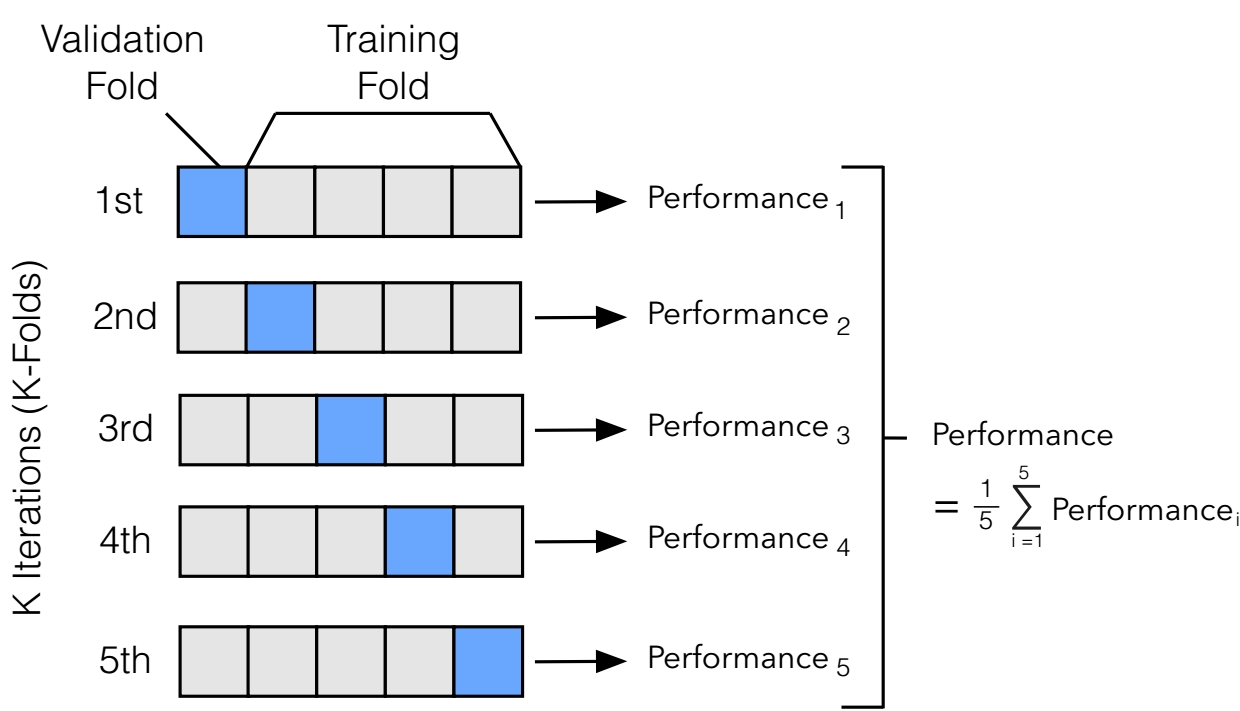
\includegraphics[width=0.7\linewidth]{img/kfoldCV.jpg}
    \caption[Esempio \emph{5-fold cross-validation}.]{Tratto da~\cite{model_evaluation}. Esempio di come \emph{5-fold cross validation} suddivide i dati di addestramento disponibili in 5 parti, utilizzandole tutte una volta come \emph{test} (i riquadri blu).}
    \label{fig:kfoldcv}
\end{figure}
Si parla di \emph{stratified k-fold cross-validation} quando la procedura mantiene la proporzione delle etichette originali nel creare le diverse suddivisioni.


\section{Selezione dei modelli}\label{sec:model_selection}
L'addestramento di un modello di apprendimento automatico richiede il più delle volte la scelta di un valore per alcuni iperparametri. 
Nel caso dei modelli \emph{k-nearest neighbours} (descritti in seguito nel~\Cref{sec:ml:knn}), per esempio, è necessario fissare un valore per il parametro $k$. 
La scelta di questi eventuali iperparametri è di assoluta importanza, ma non esiste una regola generica ed automatica per fissare a priori un valore soddisfacente. La scelta dei valori potrebbe dipendere da tanti fattori, come per esempio dalle caratteristiche dei dati a disposizione, oppure dagli obiettivi desiderati (per esempio potrebbe essere preferibile un modello che genera pochissimi falsi negativi a scapito di più falsi positivi).
In genere, si utilizzano dei criteri o degli algoritmi per selezionare le migliori combinazioni di iperparametri per il problema da risolvere: questa fase nel processo di creazione di un modello di addestramento automatico è chiamata \emph{model selection}.
Le tecniche di \emph{model selection} richiedono molteplici esecuzioni dell'algoritmo di addestramento e altrettante valutazioni su un insieme di dati che non può però essere l'insieme di \emph{test}, dato che è riservato per la valutazione finale di un modello. 
L'insieme di \emph{test} simula dei dati mai visti dal modello per stimare la bontà di generalizzazione e non può essere utilizzato per aggiustare gli iperparametri.
In caso lo fosse si verificherebbe lo scenario chiamato come \emph{data leakage}, ovvero l'utilizzo durante l'addestramento di informazioni che non dovrebbero essere usate per non falsare la bontà del modello.
Si descrivono in questo paragrafo le principali tecniche di \emph{model selection}, mentre in~\cite{model_evaluation} si può trovare una descrizione esaustiva.

I prossimi due paragrafi descrivono rispettivamente le tecniche di identificazione dei migliori valori per gli iperparametri e la problematica del \emph{bias} pessimistico.

\subsubsection{Combinazioni di valori degli iperparametri}
I possibili valori per ogni iperparametro sono definiti in una griglia di iperparametri.
In base ai possibili valori che vengono provati nella procedura di selezione del miglior modello, si identificano diverse strategie di \emph{grid search}, ovvero procedure per provare le varie combinazioni di parametri, tra cui le seguenti.
\begin{itemize}
    \item \emph{Grid search} esaustiva, in cui si provano tutte le possibili combinazioni di iperparametri. \`E la strategia più semplice ma anche la più costosa dal punto di vista computazionale, perché è sostanzialmente una ricerca a forza bruta.
    \item \emph{Randomized grid search}~\cite{random_grid_search}, in cui si selezionano casualmente dei sottoinsiemi delle possibili combinazioni di iperparametri da provare. Il risultato potrebbe variare tra diverse esecuzioni e non c'è la garanzia di trovare la miglior combinazione tra i valori della griglia.
    Ciò nonostante questa strategia può comunque fornire un buon risultato e rimane una buona opzione da considerare nei casi in cui una ricerca esaustiva non sia fattibile. 
\end{itemize}


\subsubsection{Bias pessimistico} Il termine \emph{bias} pessimistico indica che la valutazione delle capacità di generalizzazione effettuata su un sottoinsieme dei dati disponibili possa essere troppo pessimistica rispetto alle capacità che si sarebbero potute ottenere addestrando il modello sull'intero insieme di dati~\cite{model_evaluation}.
Purtroppo, utilizzare tutti i dati disponibili per addestrare il modello renderebbe inaffidabile qualsiasi valutazione effettuata con gli stessi (a causa del \emph{data leakage}); si preferisce di solito una valutazione pessimistica che una ottimistica.


\subsection{Triplo hold-out}
Si è già discusso di come il \emph{dataset} di \emph{test} non possa essere utilizzato per trovare i migliori iperparametri per un modello.
Un primo approccio è quello di suddividere in modo leggermente diverso l'insieme totale dei dati a disposizione, prevedendo 3 sottoinsiemi, descritti nell'elenco seguente.
\begin{itemize}
    \item Insieme di addestramento (\emph{train set}): utilizzato per addestrare i modelli.
    \item Insieme di validazione (\emph{validation set}): utilizzato per valutare i modelli con lo scopo di definire i migliori iperparametri.
    \item Insieme di \emph{test} (\emph{test set}): utilizzato in ultima battuta per stimare l'errore di generalizzazione.
\end{itemize}
Questa suddivisione in tre parti è chiamata \emph{triplo hold-out}.

La selezione di un insieme di validazione è critica tanto quanto la selezione dell'insieme di \emph{test}.
La procedura di selezione del miglior modello procede applicando i passi seguenti.
\begin{enumerate}
    \item Per ogni combinazione di parametri che si desidera valutare, si addestra un modello sull'insieme di addestramento e lo si valuta sull'insieme di validazione.
    \item Si utilizzano gli iperparametri che al passo precedente hanno generato il modello più performante per addestrare un nuovo modello sull'unione dei dati di addestramento con i dati di validazione, cercando così di ridurre il \emph{bias} pessimistico.
    \item Si misura la bontà di questo ultimo modello sui dati di \emph{test}.
\end{enumerate}

\subsection{Hold-out e cross-validation}
Estendendo l'approccio presentato nel paragrafo precedente, è possibile integrare la tecnica di \emph{cross-validation} nel processo di selezione dei migliori iperparametri, utilizzando il procedimento seguente.
\begin{enumerate}
    \item Si suddividono i dati in due insiemi: addestramento e \emph{test}.
    \item Per ogni combinazione di parametri che si desidera valutare, si addestra un modello sull'insieme di addestramento utilizzando \emph{cross-validation} per valutarne la bontà.
    \item Si selezionano gli iperparametri che hanno generato al passo precedente il modello più performante, e si addestra un nuovo modello sull'intero insieme di addestramento.
    \item Si misura infine sui dati di \emph{test} la bontà del modello addestrato al passo precedente.
\end{enumerate}
In questa procedura, al contrario del triplo \emph{hold-out}, non esiste un insieme di validazione fisso, perché viene utilizzata invece \emph{cross-validation}, ottenendo in questo modo una valutazione più affidabile dell'efficacia delle combinazioni di parametri.
L'insieme di \emph{test}, come al solito, viene utilizzato esclusivamente alla fine del processo per stimare l'errore di generalizzazione su dati mai visti.

\subsection{Nested cross-validation}
La \emph{nested cross validation} estende ulteriormente l'approccio visto nel paragrafo precedente.
Invece che utilizzare un solo insieme di test, si utilizza un'ulteriore procedura di \emph{cross validation} per stimare l'errore di generalizzazione.
Per questo motivo si chiama ``annidata'': ogni addestramento eseguito utilizzando le $k-1$ fold di addestramento è a sua volta eseguito con un ulteriore procedura di \emph{cross-validation}.
In~\Cref{fig:nested_cv} si riporta un illustrazione del funzionamento.
\begin{figure}
    \centering
    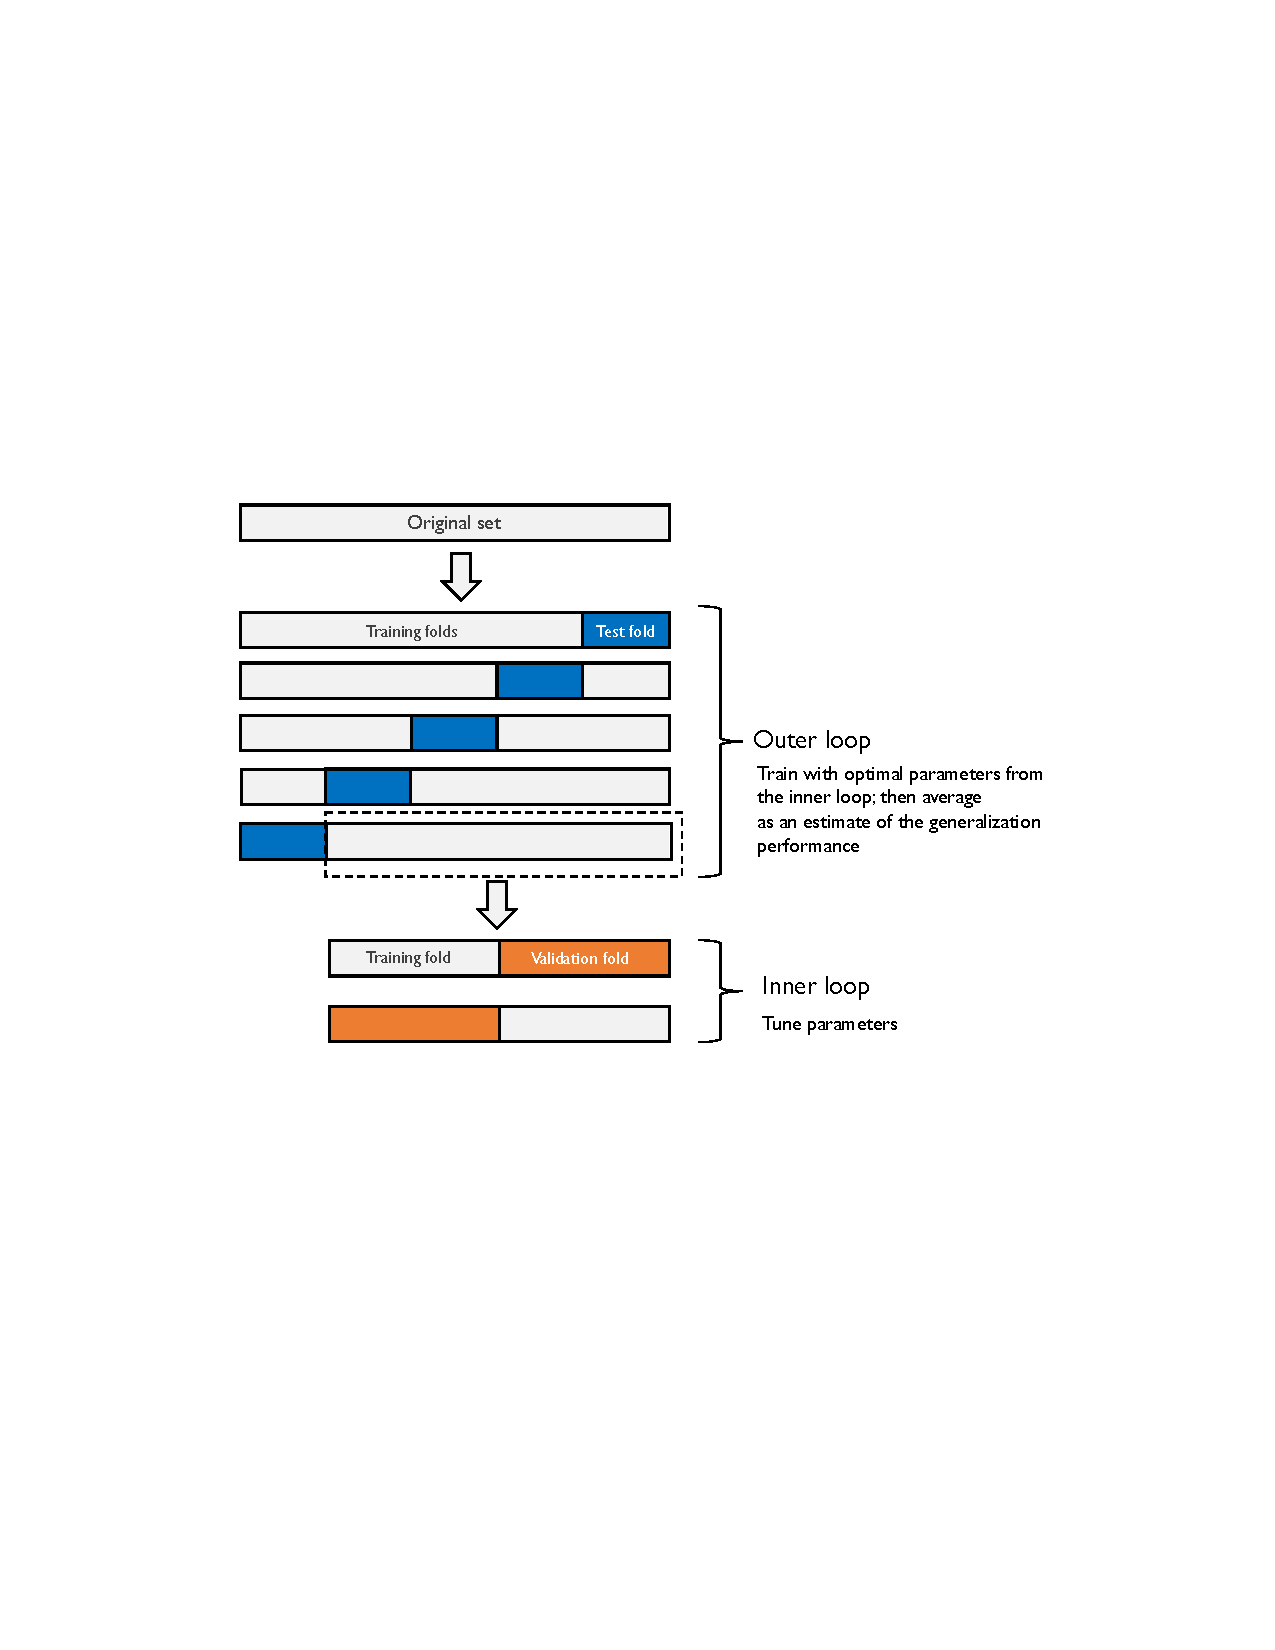
\includegraphics[width=0.8\linewidth]{img/nested_cv.pdf}
    \caption[Esempio \emph{nested cross-validation}.]{Tratto da~\cite{model_evaluation}, esempio di \emph{nested cross-validation}.}
    \label{fig:nested_cv}
\end{figure}

\section{Comuni approcci risolutivi}\label{sec:comuni_approcci_risolutivi}
In questo paragrafo si descrivono brevemente alcuni algoritmi comunemente utilizzati per risolvere i problemi tipici dell'apprendimento automatico categorizzati nel~\Cref{sec:tipi_problemi_ml}.
I modelli \emph{support vector machine}, che sono oggetto specifico del lavoro di tesi, saranno invece descritti in dettaglio nel~\Cref{chap:SVC}.

\subsection{K-Nearest Neighbors}\label{sec:ml:knn}
\emph{K-Nearest Neighbors} (KNN), descritto in dettaglio in~\cite{KNN}, è un algoritmo di apprendimento automatico che può essere utilizzato sia per problemi di classificazione che  per problemi di regressione. 
L'idea alla base del funzionamento è quella di predire un etichetta (continua o discreta) basandosi su una misura di vicinanza per i punti dell'insieme di addestramento. 
Secondo questa caratteristica, così come i modelli \emph{support vector machine} che si vedranno in seguito, anche KNN è un \emph{instance based learner}, ovvero un modello definito da un sottoinsieme di dati di addestramento, utilizzati per fare predizioni su nuovi dati.

Per problemi di classificazione binaria e multi-classe, fissato un intero $K$, KNN individua i $K$ punti dati più vicini a un punto sconosciuto $\Vec{x}_\text{new}$. 
La classe più comune tra questi vicini diventa la classe prevista per il punto $\Vec{x}_\text{new}$. 
In~\Cref{fig:knn_example} si mostra un esempio di classificazione, con $K=3$.
\begin{figure}
    \centering
    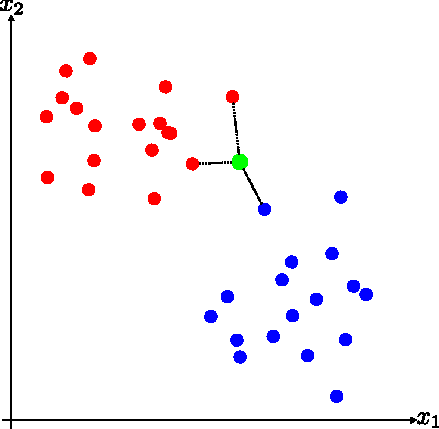
\includegraphics[width=0.7\linewidth]{img/KNN.pdf}
    \caption[Esempio \emph{K-Nearest Neighbors}.]{Esempio di applicazione della regola di classificazione KNN con $K=3$. I colori blu e rosso identificano le due possibili classi. Il punto color verde è il punto per cui predire la classe.
    Il nuovo punto sarà predetto come appartenente alla classe rossa, perché la maggioranza dei dei tre punti a lui più vicini (evidenziati dai segmenti tratteggiati) appartiene a quella classe.}
    \label{fig:knn_example}
\end{figure}

Per problemi di regressione, invece, si calcola la predizione per un punto $\Vec{x}_\text{new}$ come media dei valori dei $K$ punti vicini.

L'utilizzo di un modello KNN richiede di scegliere \emph{a priori} l'iperparametro $K$:
come per altri modelli, risulta necessaria una fase di \emph{model selection} (\Cref{sec:model_selection}) per identificare i migliori iperparametri.
La funzione di misura della distanza tra i dati di addestramento è eventualmente un ulteriore iperparametro modificabile.

KNN è un algoritmo facile da comprendere e implementare, ma ha delle evidenti limitazioni. 
\`E sensibile alla scelta di $K$ ed è particolarmente inadatto per \emph{dataset} di grandi dimensioni, sia a causa dello spazio richiesto per memorizzare il modello appreso (tutti i dati di addestramento), sia (soprattutto) per il costo computazionale, dato che è necessario calcolare la distanza rispetto a ogni elemento per ogni predizione.

Nonostante queste limitazioni, KNN rimane una scelta valida da prendere in considerazione quando si analizzano \emph{dataset} di piccole dimensioni.

\subsection{Alberi di decisione}
Gli alberi di decisione~\cite{decision_tree}, sono modelli che effettuano predizioni basandosi su una struttura dati ad albero, creata durante il processo di addestramento. 
Ogni nodo dell'albero rappresenta una regola, che, valutata su un generico dato $\Vec{x}_\text{new}$, indicherà in quale sotto-albero procedere con la predizione, fino ad arrivare a una foglia che identifica la classe da assegnare. 
In~\Cref{fig:decision_tree} si mostra un esempio di albero di decisione per un problema di classificazione.
Gli alberi di decisione possono anche essere utilizzati per risolvere problemi di regressione.

Il processo di addestramento di un albero decisionale identifica quali sono le regole da utilizzare per raggiungere buone performance di classificazione. 
L'algoritmo di addestramento più noto è CART. 
In questo algoritmo, la bontà di ogni decisione, o in altre parole il criterio con cui creare i nodi interni dell'albero, viene valutata secondo una metrica, tra le più famose si annoverano: \emph{Gini impurity}, \emph{information gain} e \emph{root mean squared error (RMSE)}. 
\begin{figure}
    \centering
    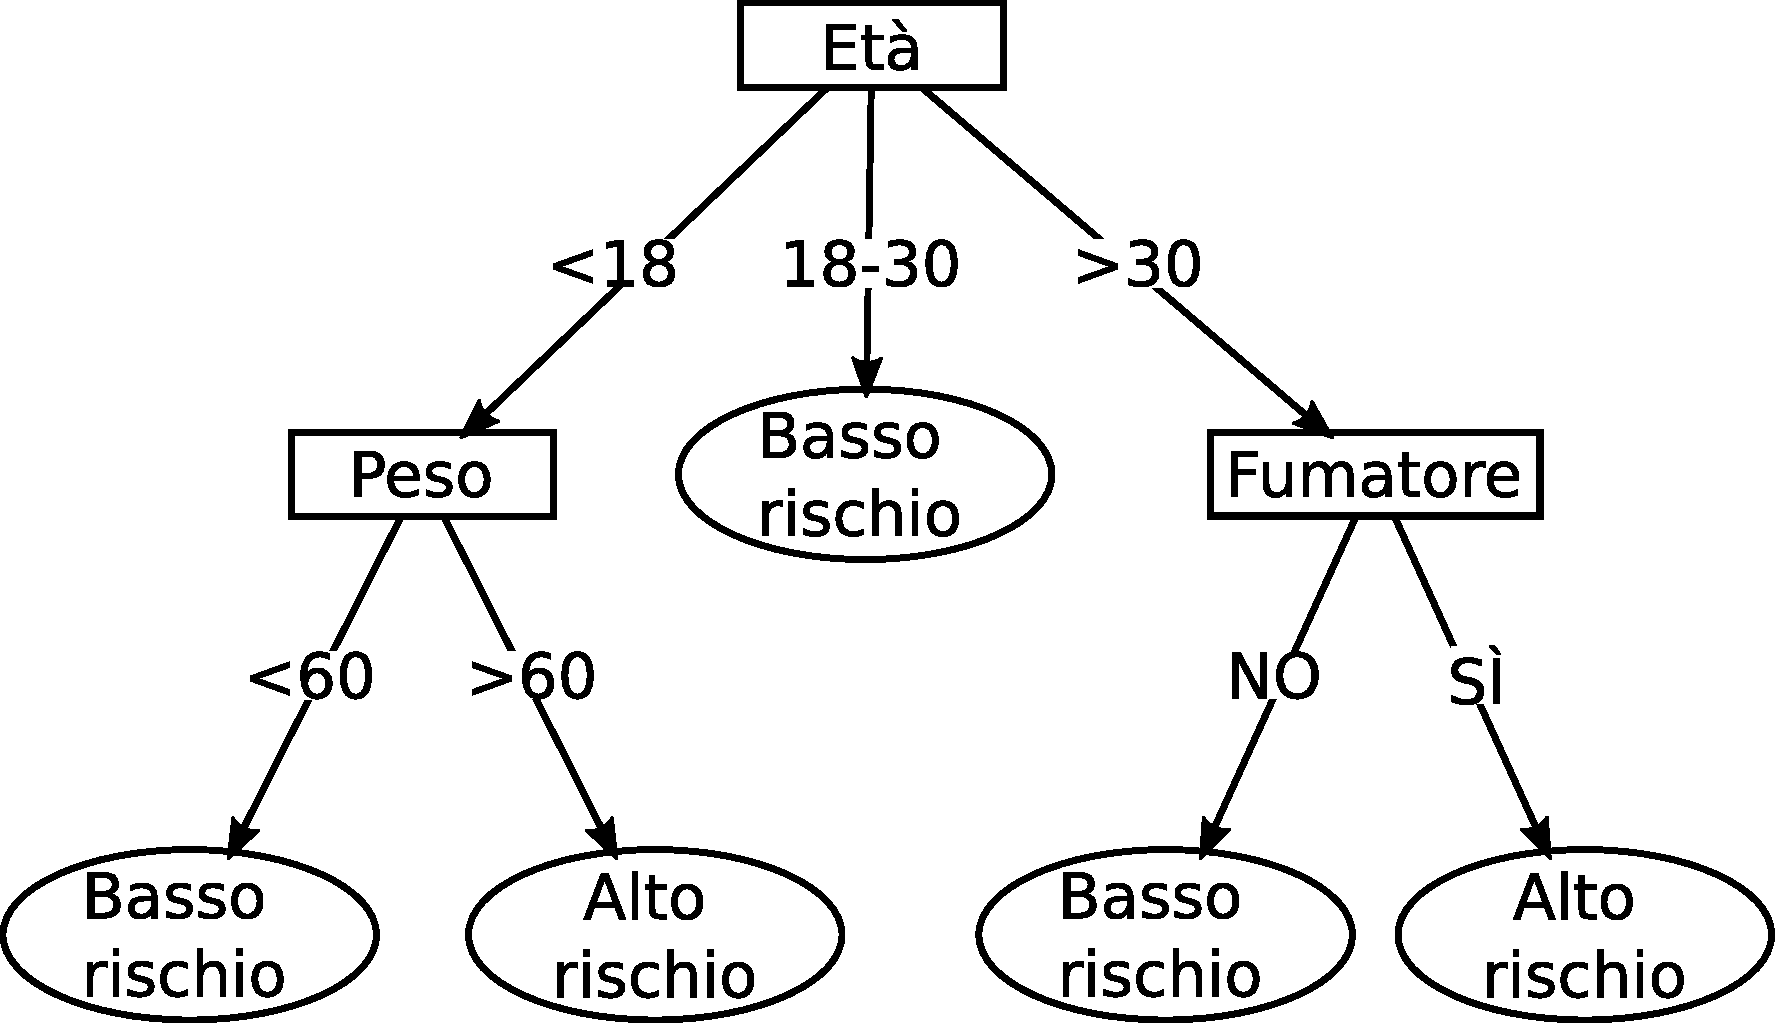
\includegraphics[width=0.7\linewidth]{img/decision_tree.pdf}
    \caption[Esempio albero di decisione.]{Esempio semplificato di un possibile albero di decisione per il rischio di malattia cardiaca. I nodi rettangolari e i corrispettivi archi che collegano ai sotto-alberi identificano delle regole, in questo caso un semplice controllo sull'attributo con il nome del nodo. I nodi foglia ovali identificano il valore della predizione.}
    \label{fig:decision_tree}
\end{figure}
Gli alberi decisionali sono modelli semplici e hanno il pregio di essere modelli \emph{white box}, ovvero sono noti i criteri per cui è eseguita una predizione.
Hanno però la tendenza a essere soggetti al fenomeno dell'\emph{overfitting} (il modello impara troppo fedelmente i dati di addestramento), dato che è sempre possibile ottenere un albero con una foglia per ogni dato di addestramento, e soffrono di \emph{variance error}, dato che anche minimi cambiamenti nell'insieme di addestramento potrebbero avere un'influenza enorme sul modello prodotto.
Queste problematiche saranno meglio discusse nel~\Cref{sec:bias_variance_tradeoff}.
Per queste limitazioni, nella pratica sono molto più utilizzati gli \emph{ensemble} di alberi decisionali, utilizzando tecniche come \emph{bagging}~\cite{bagging_predictors} e \emph{boosting}~\cite{adaboost}.
Un modello \emph{ensemble} è composto da molteplici modelli ``interni'' combinati per ottenere prestazioni migliori; non necessariamente i modelli sono omogenei.
Il tipico esempio di modello \emph{ensemble} è il modello \emph{random forest}, descritto di seguito.

\subsubsection{Random Forest}
Un primo metodo per creare un \emph{ensemble} di alberi decisionali è chiamato \emph{bagging predictors}~\cite{bagging_predictors}, termine che deriva da \emph{\textbf{b}ootstrap} \emph{\textbf{agg}regat\textbf{ing}}.
L'idea alla base del funzionamento è la seguente: il \emph{dataset} di addestramento originale $D$ viene utilizzato per creare $k$ ulteriori \emph{dataset} di dimensioni minori (circa $\frac{2}{3}$ del \emph{dataset} originale) contenenti elementi estratti da $D$ uniformemente a caso con ripetizione.
Su questi $k$ \emph{dataset} si addestrano (singolarmente) altrettanti alberi di decisione, per poi creare un modello unico che aggrega le loro predizioni utilizzando una regola sensata per il problema trattato: per un problema di classificazione, per esempio, si potrebbe utilizzare un voto di maggioranza.

I modelli \emph{random forest}~\cite{random_forest} estendono l'approccio \emph{bagging} introducendo anche la randomizzazione degli attributi. 
Ognuno dei $k$ modelli interni sarà addestrato su un sottoinsieme  di attributi, selezionati casualmente senza ripetizione, una sola volta per l'intero albero oppure a ogni creazione di un nodo interno.
Le predizioni sono poi aggregate come nei \emph{bagging predictors}.
In~\Cref{fig:random_forest} si mostra un esempio schematico di un \emph{ensemble} di alberi.

\begin{figure}
    \centering
    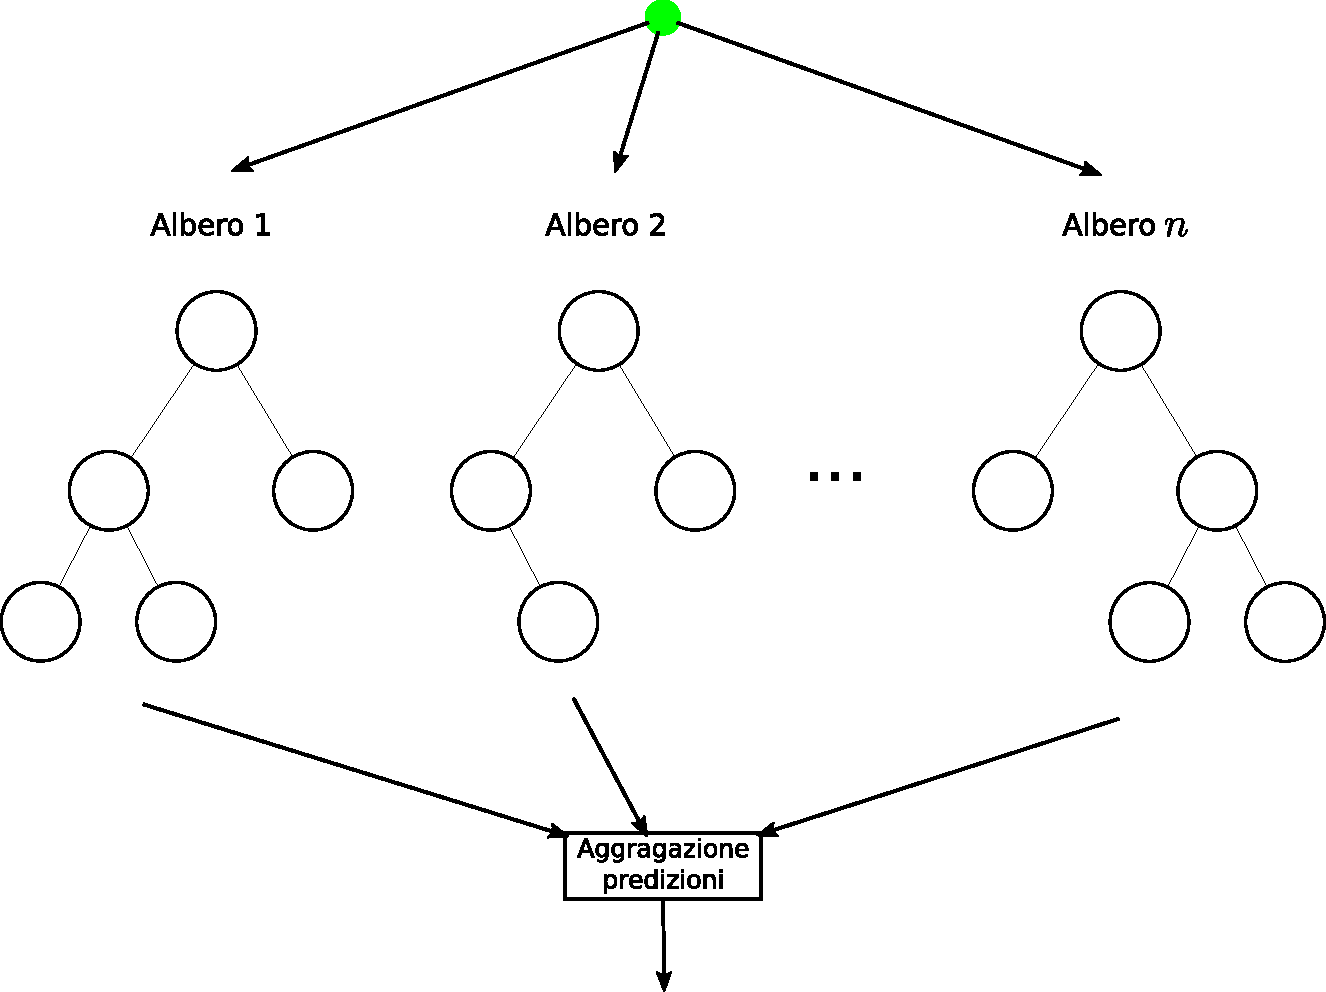
\includegraphics[width=0.7\linewidth]{img/random_forest.pdf}
    \caption[Esempio \emph{random forest}.]{Esempio di \emph{random forest}. Il modello è composto da un insieme di alberi interni, ognuno addestrato su un diverso sottoinsieme di dati e di attributi. Un nuovo esempio da classificare, in questa figura il punto verde, viene classificato da ogni sotto-albero singolarmente, per poi produrre una predizione globale utilizzando una regola di aggregazione delle predizioni interne.}
    \label{fig:random_forest}
\end{figure}

\subsubsection{Boosting}
Un altro approccio per creare \emph{ensamble} di alberi è quello che sfrutta la tecnica chiamata \emph{boosting}, che consiste nel combinare molteplici \emph{weak learner} (in questo caso alberi decisionali molto semplici, anche un solo nodo interno) in modo da ottenere, combinandoli tra loro, uno \emph{strong learner}, ovvero un modello in grado di trattare problemi complessi.
Relativamente agli alberi di decisione gli approcci più famosi sono \emph{AdaBoost}~\cite{adaboost} e \emph{XGboost}~\cite{xgboost}.

%\subsection{Logistic regression}

\subsection{Reti neurali}
Le reti neurali, descritte in dettaglio in~\cite{neural_networks}, sono un tipo di modello di apprendimento automatico ispirato alla struttura del sistema nervoso centrale umano.
Questi modelli imitano il modo in cui i neuroni biologici si scambiano impulsi.
Nella categoria reti neurali rientra una quantità di modelli molto ampia e varia.

Un primo modello di rete neurale è il modello \emph{perceptron} (percettrone)~\cite{1958_perceptron}; viene riportato un esempio in~\Cref{fig:perceptron}.
Un percettrone è un modello di molto semplice composto da un singolo neurone artificiale.
Il neurone riceve in ingresso un vettore $\Vec{x}=[x^{(1)},\dots,x^{(d)}]$ con $\Vec{x} \in \mathbb{R}^d$ ed emette un \emph{output} 
\begin{equation*}
    \hat{y} = \theta\left(\sum_{j=1}^{d}x^{(j)}w^{(j)} +b\right),
\end{equation*} 
dove $w^{(1)},\dots,w^{(d)} \in \mathbb{R}$ sono chiamati pesi, $b \in \mathbb{R}$ è la soglia e $\theta$ è la \emph{funzione di attivazione}, che nel percettrone originale è la \emph{step function} 
\begin{equation*}
    \sigma(x) =
    \begin{cases*}
      1 & se $x>0$, \\
      0 & se $x\leq0$.
    \end{cases*}
\end{equation*}
\begin{figure}
    \centering
    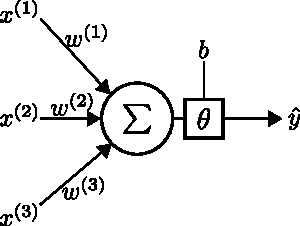
\includegraphics[width=0.3\linewidth]{img/perceptron.pdf}
    \caption[Esempio percettrone.]{Esempio di percettrone. I simboli $x^{(1)},x^{(2)},x^{(3)}$ identificano gli \emph{input}, mentre $\hat{y}$ denota l'\emph{output} del modello. I parametri $w^{(1)},w^{(2)},w^{(3)}$ sono i pesi, mentre $b$ è la soglia opzionale e $\theta$ è la funzione di attivazione.}
    \label{fig:perceptron}
\end{figure}
Il percettrone è un modello semplice, in grado di calcolare funzioni all'interno di una classe piuttosto limitata e quindi non particolarmente espressiva.
Tuttavia, è il modello alla base per la creazione di reti neurali più complesse, come per esempio il percettone multi-strato.

Il percettrone multi-strato è una rete neurale composta da molteplici percettroni collegati tra loro e organizzati in più strati: strato di \emph{input}, uno o più strati nascosti e uno strato di \emph{output}. Si mostra in~\Cref{fig:NN} un esempio di questo tipo di rete. 
A differenza del percettrone, i neuroni delle reti multi-strato utilizzano una funzione di attivazione 
diversa, per esempio la funzione \emph{ReLU} o una funzione sigmoidea.
A seconda del numero di strati nascosti è possibile suddividere questi modelli in \emph{shallow} se con pochi strati o \emph{deep} se con molti strati.
\begin{figure}
    \centering
    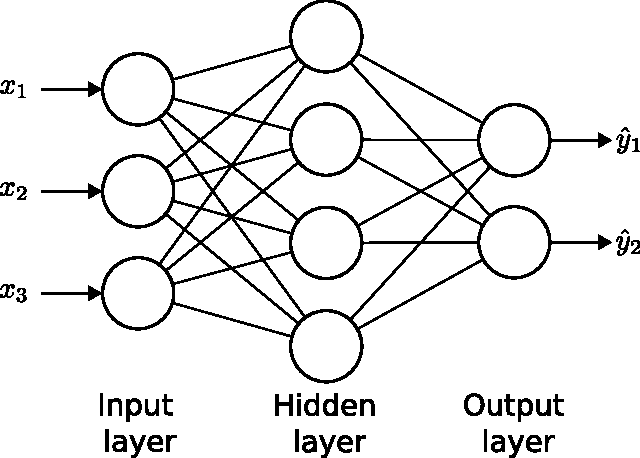
\includegraphics[width=0.5\linewidth]{img/nn.pdf}
    \caption[Esempio percettrone multi-strato.]{Esempio di un semplice percettrone multi-strato con tre neuroni di \emph{input} e due di \emph{output}.}
    \label{fig:NN}
\end{figure}
Le reti neurali descritte fino a ora sono chiamate \emph{feed-forward} perché i dati in fase di predizione fluiscono dallo strato di \emph{input} fino a quello di \emph{output}.
Esistono altre tipologie di reti con strutture più complesse, per esempio le reti ricorrenti, le reti convoluzionali, le reti generative e altre numerose varianti~\cite{aggarwal2018neural}.
In generale, una rete neurale più complessa è composta da molteplici neuroni artificiali, non per forza percettroni; come accennato in precedenza, l'insieme di modelli reti neurali è vasto e variegato.

L'addestramento di una rete neurale \emph{feed-forward} è effettuato con l'algoritmo di retro-propagazione dell'errore~\cite{neural_networks}.
Nella prima fase, \emph{forward-pass}, un insieme di dati passa nella rete fino a produrre le predizioni corrispondenti, per le quali si calcola l'errore. In seguito, percorrendo a ritroso la rete in una fase \emph{backwards-pass}, si aggiustano i pesi e la soglia dei neuroni in modo da ridurre l'errore misurato.
Queste due fasi permettono di calcolare le derivate di una funzione di perdita (per esempio l'accuratezza) rispetto ai pesi e ai bias dei vari neuroni: i valori di queste derivate vengono poi utilizzati per eseguire l'algoritmo del gradiente, col risultato di ottimizzare la funzione di perdita.

In base alla tipologia di rete neurale esistono diversi algoritmi di addestramento, ma in generale si utilizza un metodo del gradiente per ridurre iterativamente l'errore sui dati di addestramento.

L'algoritmo procede iterativamente fino al verificarsi di una condizione di arresto, per esempio il superamento di un numero massimo di istruzioni, o il raggiungimento di un errore di predizione sufficientemente basso.

\section{Bias-variance tradeoff}\label{sec:bias_variance_tradeoff}
Il termine \emph{bias-variance tradeoff}~\cite{elements-of-statistical-learning} si riferisce a una caratterizzazione dell'errore di generalizzazione, ovvero la discrepanza tra i valori effettivi e quelli predetti, relativamente a un insieme di \emph{test} e alle relative implicazioni pratiche.

Il concetto può essere formalizzato come in~\cite{elements-of-statistical-learning}, ma ci si limiterà in questo paragrafo a descriverlo sinteticamente con un esempio.
Si ipotizzi di avere disponibile un \emph{dataset} con le caratteristiche di alcuni pazienti: si pone il compito di costruire un modello per predire se una data persona è a rischio di soffrire di infarto oppure no.
Si consideri ora di costruire un modello molto semplice: un albero di decisione composto da un solo nodo, per cui se l'età del paziente è $>50$ si predice ``rischio alto'', altrimenti si predice ``rischio basso''.
Un modello di questo tipo ha \emph{variance} molto bassa, perché tutto sommato poco sensibile a piccoli cambiamenti nei dati di addestramento. Un paziente con sessanta anni di età ha lo stesso rischio di un paziente con sessanta anni e un giorno di età.
Di contro, questo modello ha \emph{bias} molto alto, perché esegue la predizione solo ed esclusivamente controllando l'età del paziente, evitando di considerare tutte le altre importanti informazioni, facendo di fatto delle assunzioni troppo semplicistiche sulla funzione da approssimare. 
Questo modello non è in grado di approssimare la relazione reale espressa dai dati.
Cambiando approccio, si ipotizzi invece di addestrare un albero di decisione molto profondo, arrivando a generare un nodo foglia per ogni dato di addestramento.
Questo secondo modello avrà \emph{bias} molto basso, perché non farà assunzioni sulla funzione da modellare, anzi ogni possibile attributo sarà valutato per decidere che ramo seguire; allo stesso tempo avrà \emph{variance} molto alta, perché anche una piccola variazione nel dato di \emph{input} risulterà in un percorso nell'albero diverso, ottenendo una predizione potenzialmente molto diversa.
In questo caso, il rischio predetto per un paziente con sessanta anni di età potrebbe essere molto diverso dal rischio predetto per un paziente con sessanta anni e un giorno di età.
Anche questo modello non è in grado di approssimare la relazione reale espressa dai dati in modo soddisfacente.

Un modello con buone capacità di generalizzazione deve esibire basso \emph{bias} e bassa \emph{variance}. Si utilizza il termine \emph{bias-variance tradeoff} (compromesso appunto) perché è molto difficile minimizzare entrambe queste caratteristiche contemporaneamente. In genere, implementare delle tecniche per migliorare il \emph{bias} fa peggiorare la \emph{variance} e viceversa.
Nonostante ciò, è spesso possibile trovare un modello con buone capacità di generalizzazione. 

Questo problema si traduce nella pratica nel problema di \emph{overfitting} e \emph{underfitting}.
Un modello che soffre di \emph{overfitting} (alta \emph{variance}, basso \emph{bias}) è un modello che si è adattato troppo fedelmente ai dati di addestramento, esibendo pessime performance di generalizzazione. 
Un modello che soffre di \emph{underfitting} (alto \emph{bias}, bassa \emph{variance}) è un modello che non è sufficientemente complesso per modellare le relazioni espresse nei dati ed esibisce pessime performance di generalizzazione.
In~\Cref{fig:esempio_underfitting_overfitting} si visualizza un esempio dei vari scenari: \emph{overfitting}, \emph{underfitting} e un esempio di modello con buone capacità di generalizzazione.
\begin{figure}
    \begin{subfigure}[t]{.45\textwidth}
        \centering
        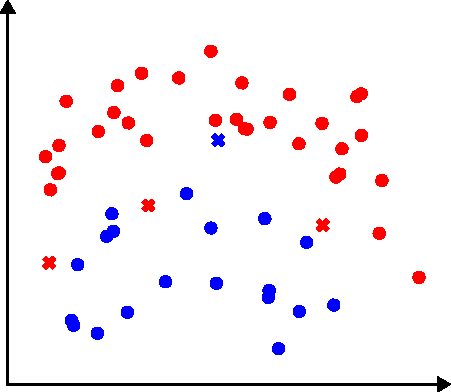
\includegraphics[width=\textwidth]{img/under_over_fitting_1.pdf}
        \caption{Dati di addestramento disponibili. Il colore identifica la classe; i punti scorrettamente etichettati sono indicati con il simbolo x.}
    \end{subfigure}%
    \hfill
    \begin{subfigure}[t]{.45\textwidth}
        \centering
        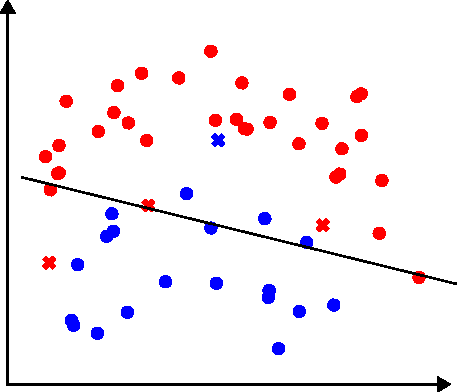
\includegraphics[width=\textwidth]{img/under_over_fitting_2.pdf}
        \caption{Esempio di come un modello lineare potrebbe esibire \emph{underfitting}.}
    \end{subfigure}%
\vskip\baselineskip
    \begin{subfigure}[t]{.45\textwidth}
        \centering
        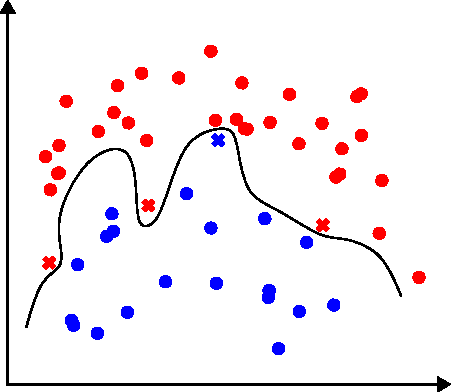
\includegraphics[width=\textwidth]{img/under_over_fitting_3.pdf}
        \caption{Esempio di come un modello non lineare potrebbe esibire \emph{overfitting}.}
    \end{subfigure}%
    \hfill
    \begin{subfigure}[t]{.45\textwidth}
        \centering
        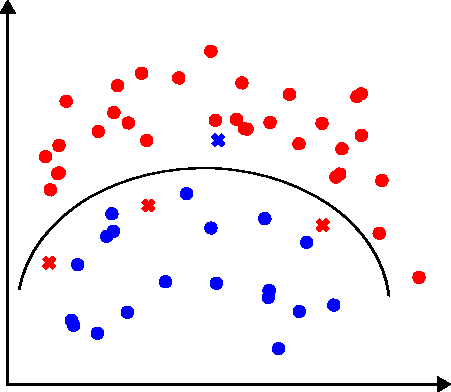
\includegraphics[width=\textwidth]{img/under_over_fitting_4.pdf}
        \caption{Esempio di una possibile superficie di separazione con buone capacità di generalizzazione.}
    \end{subfigure}%
\caption[Esempio di \emph{underfitting} e \emph{overfitting}.]{Esempio di \emph{underfitting} e \emph{overfitting} su un \emph{dataset} per un problema di classificazione binaria.}
\label{fig:esempio_underfitting_overfitting}
\end{figure}